\section{Element wise sum}
\subsection{Aim}
To find the element wise of two arrays

\subsection{Code}
\begin{lstlisting}
DATA SEGMENT
  arr1 DW 1000H, 2000H, 3000H, 4000H
  arr2 DW 4000H, 3000H, 2000H, 1000H
  sum DW 4 DUP(?)
  count DW 4
DATA ENDS

CODE SEGMENT
ASSUME CS:CODE, DS:DATA
START:
  MOV AX, DATA
  MOV DS, AX
  MOV CX, count
  LEA SI, arr1
  LEA DI, arr2
  LEA BX, sum

SUMLOOP:
  MOV AX, [SI]
  ADD AX, [DI]
  MOV [BX], AX
  ADD SI, 2
  ADD DI, 2
  ADD BX, 2
  LOOP SUMLOOP

EXIT:
  MOV AX, 4CH
  INT 21H
CODE ENDS
END START
\end{lstlisting}

\subsection{Output}
\begin{center}
	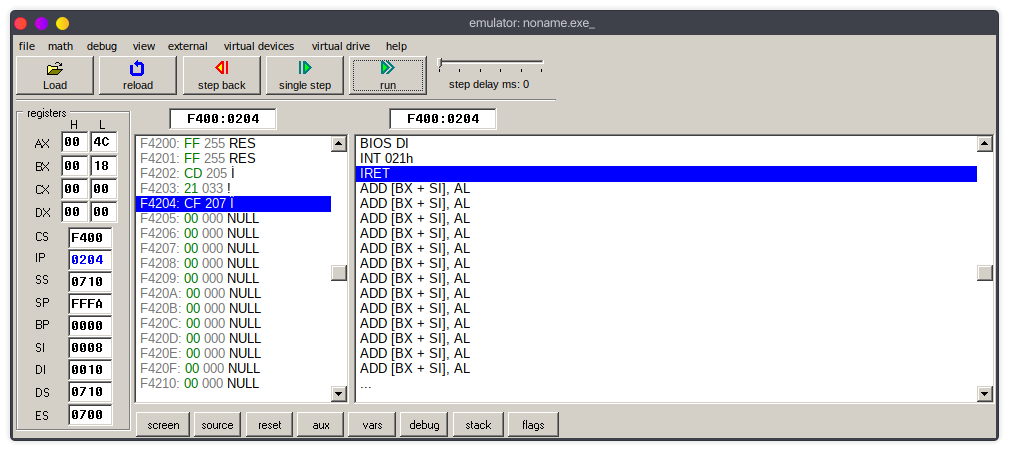
\includegraphics[width=0.90\textwidth]{img/p8/ss1.png}
	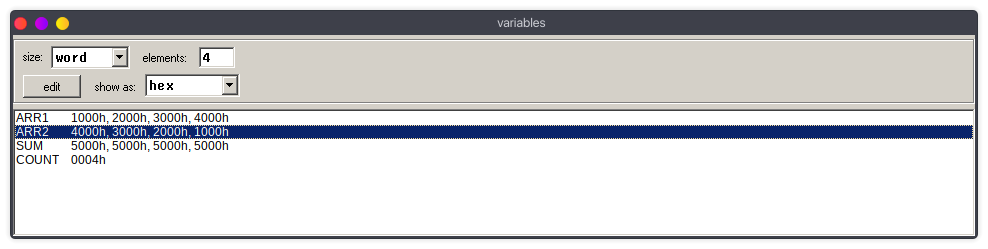
\includegraphics[width=0.90\textwidth]{img/p8/ss2.png}
\end{center}

\subsection{Result}
The element wise sum of two 32bit array was found in emu8086